\section{Paralelismo}

\begin{frame}[t]{Programación secuencial frente a paralela}
\begin{itemize}
  \item \textmark{Programación secuencial}:
    \begin{itemize}
      \item Conjunto bien conocido de \emph{estructuras de control}
            como parte de los lenguajes de programción.
      \item Estructuras de control \emph{inherentement secuenciales}
    \end{itemize}

  \vfill\pause
  \item \textmark{Programación paralela tracional}:
    \begin{itemize}
      \item Construcciones que adaptan las estructuras de control
            secuencial al mundo paralelo (p.ej. \emph{parallel-for}).
    \end{itemize}

  \vfill\pause
  \item Pero \ldots
    \begin{itemize}
      \item ¿Y si pudiesemos tener estructuras que fuesen a la vez
            secuneciales y paralelas?
    \end{itemize}
\end{itemize}
\end{frame}

\begin{frame}[t]{Diseño de software}

\begin{quote}
There are two ways of constructing a software design:\\ 
\vspace{1em}
\pause
One way is\\
\pause
to make it \textgood{so simple} that there are \textmark{obviously no deficiencies},\\
\pause
\vspace{.5em}
and the other way is\\
\pause
to make it \textgood{so complicated} that there are \textmark{no obvious deficiencies}.\\ 
\vspace{1em}
\pause
The \textmark{first method} is \textbad{far more difficult}. 
\end{quote}
\hfill C.A.R Hoare
\end{frame}

\begin{frame}[t,fragile]{Ejemplo: Transformando una secuencia}
\begin{itemize}
  \item Dada una secuencia de \cppid{frame}s, generar una 
        nueva secuencia en escala de grises.
\begin{lstlisting}
struct frame { /*...*/ };
frame togray(const frame & f);
\end{lstlisting}
\end{itemize}
\begin{center}
\input{frame-map.tkz}
\end{center}
\end{frame}

\begin{frame}[t,fragile]{Transformando una secuencia}
\begin{block}{Bucle tradicional explícito}
\lstinputlisting[firstline=6,lastline=17]{ej/src/togray/loop.cpp}
\end{block}
\end{frame}

\begin{frame}[t,fragile]{Transformando una secuencia}
\begin{block}{Al estilo STL}
\lstinputlisting[firstline=6,lastline=17]{ej/src/togray/stl-transform.cpp}
\end{block}
\end{frame}

\begin{frame}[t,fragile]{Transforming a sequence}
\begin{block}{Al estilo STL paralelo (C++17)}
\lstinputlisting[firstline=6,lastline=17]{ej/src/togray/pstl-transform.cpp}
\end{block}
\end{frame}

\begin{frame}[t]{Más allá del estándar: GrPPI}
\begin{itemize}
  \item \textgood{GrPPI}: Generic Reusable Parallel Pattern Interface.
    \begin{itemize}
      \vfill\item
      Separación de \textmark{código de aplicación} y \textmark{modelo de ejecución}.

      \vfill\item
      Composición mediante \textmark{patrones de diseño} paralelos.

      \vfill\item
      \textmark{Modelos soportados}:
        \begin{itemize}
        \item Secuencial.
        \item ISO C++ Threads.
        \item Open MP.
        \item Intel TBB.
        \item FastFlow.
        \item Dinámico.
        \end{itemize}
    \end{itemize}
\end{itemize}
\end{frame}

\begin{frame}[t]{Patrones de paralelismo}
\begin{itemize}
  \item \textgood{Patrones de datos}: Expresan cómputo sobre un conjunto de datos.
    \begin{itemize}
      \item \textmark{map}, \textmark{reduce}, \textmark{map/reduce}, \textmark{stencil}.
    \end{itemize}

  \vfill\pause
  \item \textgood{Patrones de tareas}: Expresan composiciones de tareas.
    \begin{itemize}
      \item \textmark{divide/conquer}.
    \end{itemize}

  \vfill\pause
  \item \textgood{Patrones de flujo}: Expresan cómputo sobre un flujo de datos 
        (posiblemente sin límite).
    \begin{itemize}
      \item \textmark{pipeline}.
      \item Specialized stages: \textmark{farm}, \textmark{filter}, 
            \textmark{reduction}, \textmark{iteration}.
    \end{itemize}
\end{itemize}
\end{frame}

\begin{frame}[t,fragile]{Ejemplo: Procesamiento de imagen}
\begin{block}{Mejora de imágenes}
\begin{lstlisting}
void procesa(std::istream & is, std::ostream & os) {
  grppi::parallel_omp_execution ex;

  grppi::pipeline(ex,
    [&]() -> optional<frame> {
      auto f = read_frame();
      if (is) return f;
      else return {};
    },
    grppi::discard([](const frame & f) { return f.low_quality();}),
    [](const frame & f) { return filter(f); },
    [](const frame & f) { return togray(f); },
    [&](const frame & f) { write_frame(os,f); }
  );
}
\end{lstlisting}
\end{block}
\end{frame}

\begin{frame}[t]{Resonancia Magnética Cerebral}
\begin{columns}
\column{.7\textwidth}
\begin{itemize}
  \item Método no intrusivo para acceder a la anatomía interna.
  \item Grandes cantidades de datos generadas.
  \item Aplicaciones en neurociencias.
    \begin{itemize}
      \item Desorden bipolar.
      \item Paranoia.
      \item Esquizofrenia.
    \end{itemize}
\end{itemize}

\column{.3\textwidth}
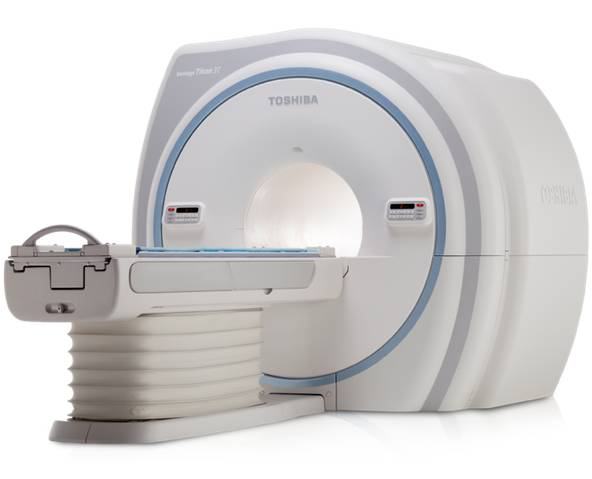
\includegraphics[width=\textwidth]{img/mri-scanner.jpg}
\end{columns}

\vspace{2em}
\begin{itemize}
  \item Identificación de fibras y conectividad entre áreas del cerebro.
\end{itemize}

\end{frame}

\begin{frame}[t]{Fibras}
\begin{center}
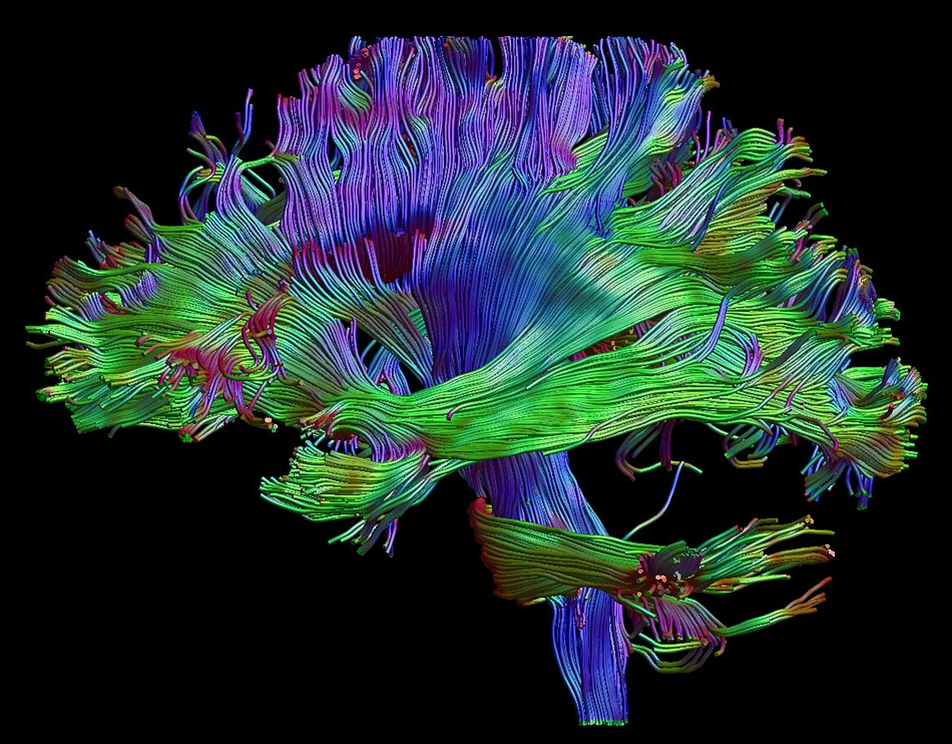
\includegraphics[width=.8\textwidth]{img/brain.png}
\end{center}
\end{frame}

\begin{frame}[t]{Evaluación}
\begin{center}
\includegraphics[width=\textwidth]{img/grppi-phardi.pdf}
\end{center}
\end{frame}

\begin{frame}[t]{Para saber más}
\begin{itemize}
  \item \textmark{C++ Concurrency in Action 2nd Edition}.
        Anthony Williams.
        Manning. 2019.

  \item \textmark{A Generic Parallel Pattern Interface for Stream and Data Processing}. 
        D. Rio, M. F. Dolz, J. Fernández, J. D. García. 
        Concurrency and Computation: Practice and Experience, 29(24): 12pp.
        2017.

  \item \textmark{Towards Automatic Parallelization of Stream Processing Applications}.
         M. F. Dolz, D. Rio, J. Fernández, J. D. García, J. Carretero. 
         IEEE Access. 6:39944–39961. 2018.
    
\end{itemize}
\end{frame}
